\chapter{Development}
\label{ch:dev}

%\begin{chapterquote}{Ludwig Wittgenstein}
%	The limits of my language mean the limits of my world.
%\end{chapterquote}
In this section we will explain the data used for the experiments as well as the process of preprocessing.

\section{Data description}
The data used in this study includes the closure stock market prices of \textit{Wal-Mart de México, S.A.B. de C.V.} known as WALMEX. The data was extracted from Yahoo! Finance applying a weekly filter over a time interval: from 02/01/2012 to 16/01/2017. The result is a database with 264 weekly prices in MXN currency. The average price is \$32.72 MXN with a standard deviation of 4.32. The minimum price is \$28.09 MXN and the maximum is \$47.22 MXN. Figure \ref{fig:walmexFreq} shows the frequency of the prices by \$1 MXN interval since the data is too variable to be able of analyzing the frequency of each price. It can be seen that the interval of highest frequency includes the prices between \$34.5 to \$35.4. 

On the other hand, if we analyze the prices by the average price of each month and year it can be noticed that the years can be classified in four different intervals. Nevertheless there are no two following years that keep the same average price interval.In 2014 the lowest average price was registered and the highest appears in 2016. When analyzing by month it can be seen in Figure \ref{fig:walmexMonth} that the months can be grouped in three intervals. In this case, there are following months that remain in the same interval: from May to July and August to September. 

 
\begin{figure}
\label{fig:walmexComp}
\center
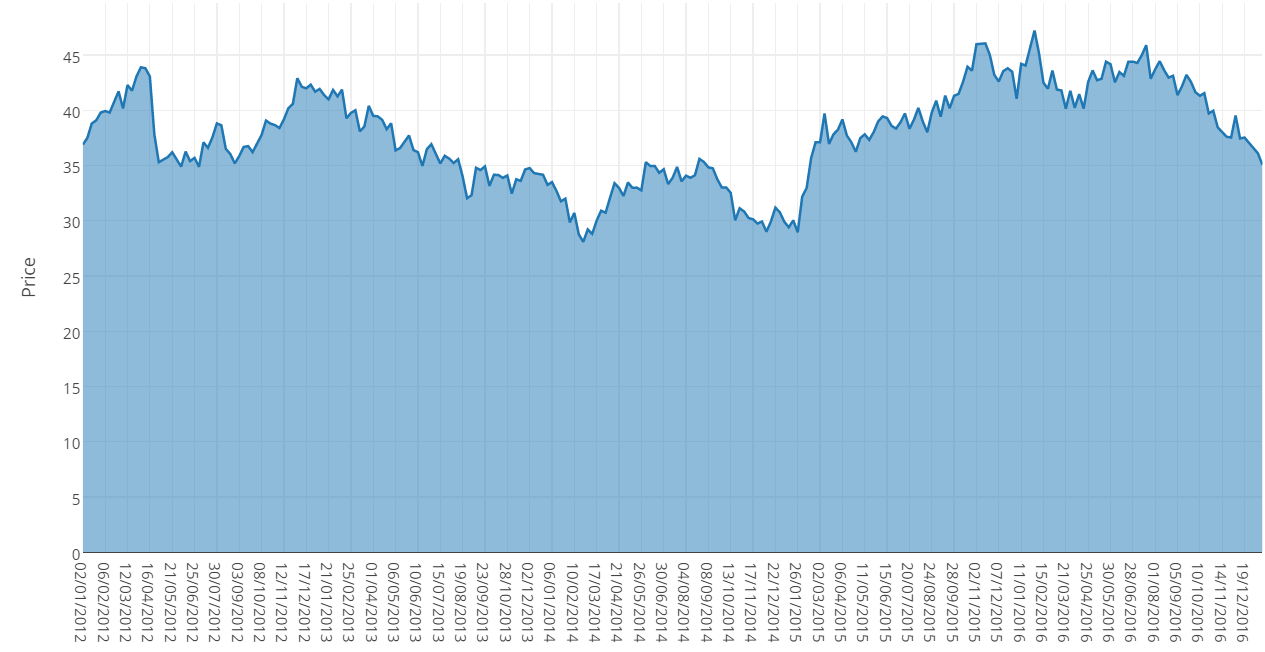
\includegraphics[width=8.5cm,height=3.5cm]{Figures/wamexCompleto.PNG}
\caption{Weekly WALMEX Stock Prices}
\end{figure}

\begin{figure}
\label{fig:walmexFreq}
\center
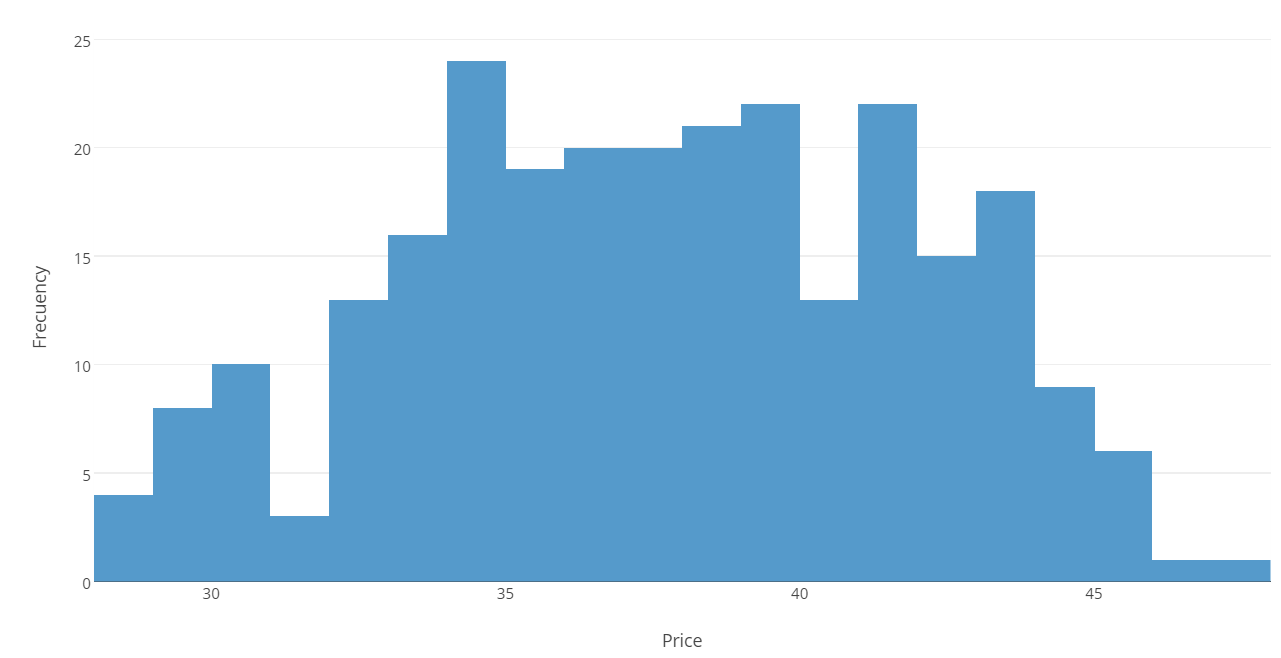
\includegraphics[width=8.5cm,height=3.5cm]{Figures/walmexHistogram.PNG}
\caption{Frequency of Prices by Intervals}
\end{figure}

\begin{figure}
\label{fig:walmexMonth}
\center
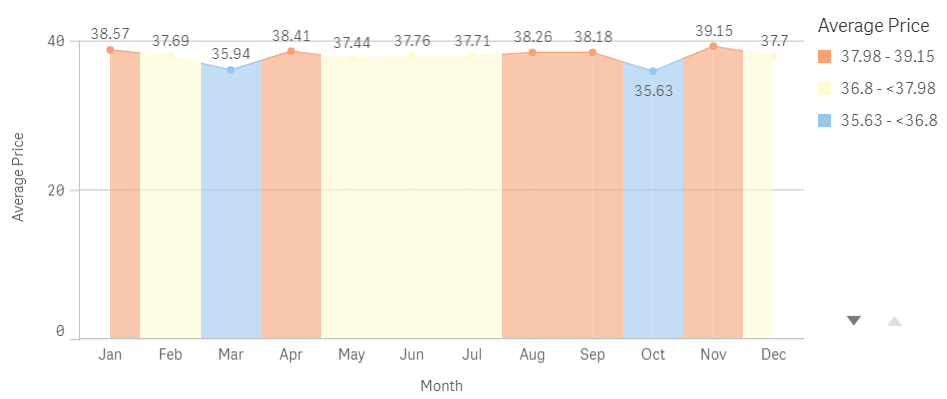
\includegraphics[width=8.5cm,height=3.5cm]{Figures/walmexMonth.PNG}
\caption{Monthly Average Stock Price}
\end{figure}

\begin{figure}
\label{fig:walmexYear}
\center
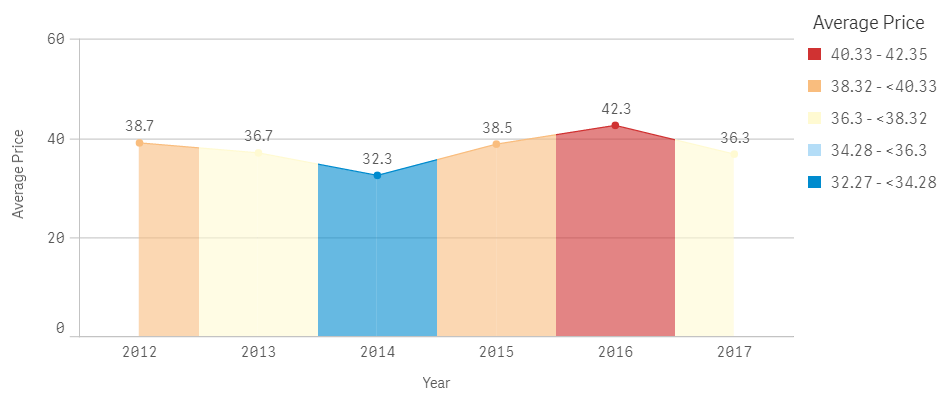
\includegraphics[width=8.5cm,height=3.5cm]{Figures/walmexYear.PNG}
\caption{Yearly Average Stock Price}
\end{figure}
\section{Preprocessing}

In this section we explain how prices are mapped to an adequate representation that the three models understand. For this task, data needs to be vectorized and we need to define the target values since the three models proposed belong to supervised learning. In this study, the preprocessing took in account three steps:

\begin{enumerate}
\item Data split
\item Normalization
\item Vectorization
\end{enumerate}

First, the database was divided in two subsets: 67\% of the data for training and the remaining 33\% for testing. Since we are working with time series, the order of the values was respected. Therefore, the first 177 prices were assigned to the training subset and the last 88 values to the testing subset. From this point, the testing subset was not occupied until the evaluation phase.

The next step was to normalize the data, meaning, the data was rescaled to the interval $[0,1]$ as follows:

\begin{equation}
\label{eq:normalize}
x_{new}=\frac{x-x_{min}}{x_{max}-x_{min}}
\end{equation}

where $x_{min}$ is the minimum value in the training subset and $x_{max}$ is the maximum values in the training subset. 

For the evaluation phase, the testing subset was also normalized taking in account the maximum and minimum value of the training subset in order to avoid adding future information to the testing subset.

In this work sequences of three prices were defined as the attributes of the database, hence, the target value is the fourth one in the sequence. Since the data is already in weekly time intervals, there is no need to keep the dates for each price. This representation gave us a training set of 173 examples and a testing set of 84. The first five examples of prive vectors with its target price are shown in table \ref{table:trainPrices}. Table \ref{table:train} exhibits the vectors after normalization.


\begin{table}{}
\begin{center}
\begin{tabular}{ c | c | c | c }
    \hline
     \textbf{Price 1} &  \textbf{Price 2} &    \textbf{Price 3} &   \textbf{TargetPrice}\\ \hline
    36.88&  37.49&  38.79 &39.09\\ \hline
    37.49&  38.79&  39.09&39.79\\ \hline
    38.79&  39.09&  39.79&39.93\\ \hline
   39.09&  39.79&  39.93&39.79\\ \hline
    39.79&  39.93&  39.790&40.72\\ \hline
    \hline
  \end{tabular}
\caption{First 5 Examples of Price Vectors}
 \label{table:trainPrices}
\end{center}

 \end{table}


\begin{table}{}
\begin{center}
\begin{tabular}{ c | c | c | c }
    \hline
    \textbf{Price 1} &  \textbf{Price 2} &    \textbf{Price 3} &   \textbf{Target Price} \\ \hline
    0.55696201 &  0.59493685&  0.6778481 &0.69620258\\ \hline
    0.59493685 &  0.6778481 &  0.69620258 &0.74050641\\ \hline
     0.6778481 &  0.69620258 &  0.74050641&0.74936712\\ \hline
     0.69620258 & 0.74050641 &  0.74936712 &0.74050641\\ \hline
     0.74050641 &  0.74936712 &  0.74050641 &0.79936719\\ \hline
    \hline
  \end{tabular}
\caption{Price Vectors after Normalization}
\end{center}
\label{table:train}
 \end{table}
 